%\documentclass[aps, prl, preprint, groupedaddress]{revtex4-1}
\documentclass[aps, prl, twocolumn, groupedaddress]{revtex4-1}

\usepackage{amsmath}
\usepackage{graphicx}  % Include figure files
\usepackage{dcolumn}   % Align table columns on decimal point
\usepackage{bm}        % bold math
\usepackage{braket}
\begin{document}

%\preprint{APS/123-QED}

\title{Generalized model for photo-induced surface structure in amorphous
  thin films}
% Force line breaks with \\

\author{Chao Lu}
\author{Daniel Recht}
\author{Craig Arnold}
\email{cbarnold@princeton.edu}
\affiliation{Princeton University}
\date{\today}

\begin{abstract}
We present a generalized model to explain the spatial and temporal
evolution of photoinduced surface structure in photosensitive
amorphous thin films. The model is constructed by employing an
incompressible viscous fluid model, driven by a photoinduced
pressure originating from dipole rearrangement. In the derivation, one
only requires the polarizability, viscosity and surface tension of
the system. We check validity of the model by fitting to experimental
data of As$_2$S$_3$ and demonstrating good agreement using two free
fitting parameters.

% The model is based on incompressible viscous
% fluid equation, combining with interaction between light radiation and
% the materials, where dipole reorientation leads to a photoinduced
% pressure.
% This model is sufficient and effective for predicting
% many aspects of photo-induced structure formation, in various
% amorphous thin films.
\end{abstract}

\pacs{Valid PACS appear here}    %PACS, the Physics and Astronomy Classification Scheme.
\keywords{chalcogenide, photoinduced surface relief, azobenzene
  polymer, viscous fluid model}
\maketitle

\section{\label{sec:intro}Introduction}
It has long been known that photoinduced surface relief structures are
generated on a variety of materials like azobenzene-containing
polymers, chalcogenides (like As$_2$S$_3$, AsSe, GeAsSe) and other
amorphous materials \cite{Viswanathan:1998jx, saliminia,
Shtutina:1995, Barada:2004dq}. Macroscopic surface structures can be
inscribed by having periodic variations in intensity or polarization
of the laser field \cite{Jiang:1998bz}. This phenomenon is potentially
useful for technologies such as rewritable optical data storage,
active optical devices, nanofabrication, and optical actuators
\cite{Kenji:2002, Kim:1995fb}. However, a complete description of the
underlying microscopic mechanism remains lacking.

In the past decades, much experimental and theoretical work has been
performed to clarify the mechanism of this phenomenon. A number of
models have been proposed to describe the formation process
\cite{saliminia, hisakuni95}, where volumetric internal pressure,
interaction among dipoles, anisotropic diffusion or optical gradient
forces have been considered as the driving force for surface
restructurings \cite{Kumar:1998je, Bian:1999ic, Lefin:1999fm}. In
spite of the efforts, a unified model to capture all experimental
observations remains lacking.

%  The main
% difficulty is how to explain the strong dependence of the matter
% motion efficiency on the light polarization.

In this paper, we develop a two-stage model, wherein we first consider
the generation of photoinduced pressure as a driving mechanism that
initiates mass transport of the film, and in the second step we study
the flow of material resulting from the application of this internal
force. The flow of material is described using the Navier-Stokes
equations for viscous flow. In this model, one assumes that the
optical-induced pressure, is large enough to provide a driving force
for mass tranport, dependent on the intensity and polarization of the
light. Finally we compare the model to the specific case of
As$_2$S$_3$, simulation shows the surface height evolution as a
function of time agrees with experimental measurements well.

\begin{figure}[!htbp]
  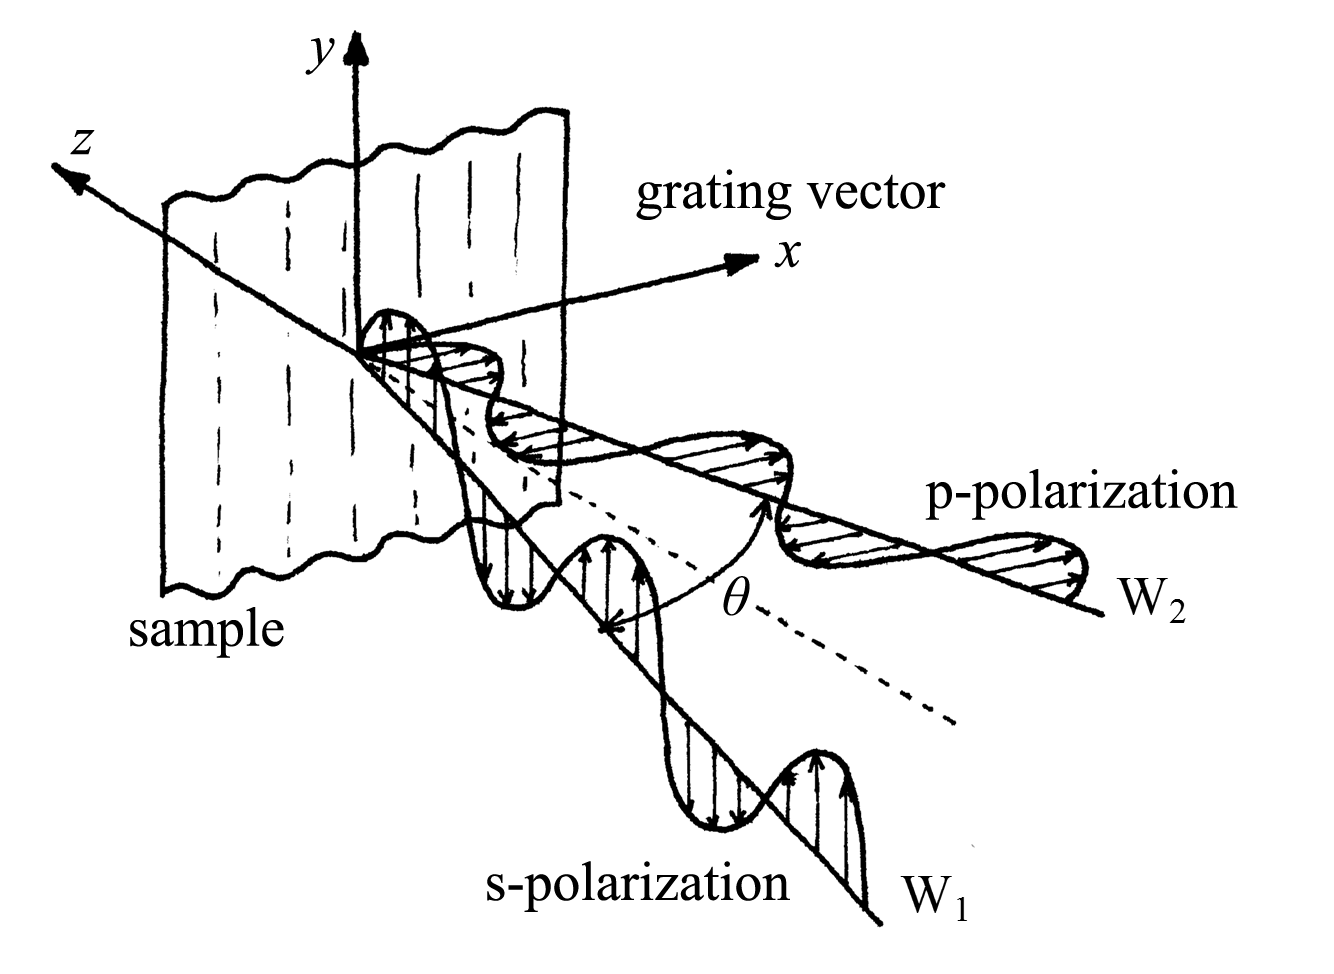
\includegraphics[width=2.45in]{figure/sppic.png}
  \caption{Schematic diagram of the typical experimental setup used to
                                                                                                                                                                                                                                                                                                                                                                                                                                                                                                                                generate surface structure.
                                                                                                                                                                                                                                                                                                                                                                                                                                                                                                                                Two beams, W1 and W2, interfere on the surface of a thin film of
                                                                                                                                                                                                                                                                                                                                                                                                                                                                                                                                amorphous light-sensitive material, leading
                                                                                                                                                                                                                                                                                                                                                                                                                                                                                                                                to the pictured definitions of the coordinate system and polarization directions.}
  \label{fig:setup}
\end{figure}

\section{The Model}
\subsection{Fluid Dynamics of Surface Relief Formation}
\label{sec:fluids}

We assume that in the presence of optical radiation, the weak
connections between the functional units in the chalcogenide glass,
i.e. the van der waals forces, is broken, allowing these units to
rearrange. Further stipulating laminar flow of the glass and
time-independent illumination that varies in one direction along the
surface (the $x$ axis) but is uniform along the other surface axis
($y$) and with depth ($z$) brings surface relief formation in the thin
films within the scope of the Navier-Stokes equation simplified into a
two-dimensional boundary layer equation in $x$ and $z$ \cite{levich}
(see figure \ref{fig:setup}).

\begin{equation}
\frac{\partial v_x}{\partial t}+v_x\frac{\partial v_x}{\partial x} +v_z\frac{\partial
v_x}{\partial z} = - \frac{1}{\rho}\frac{\partial \mathcal{P}}{\partial
x}+\nu\frac{\partial^2 v_x}{\partial z^2}+f \mathrm{,} \label{eq:levstokes}
\end{equation}

in which the $v_i$'s are components of the velocity vector, $\rho$ is
the mass density, $\mathcal{P}$ is the total pressure, $f$ is the body
force, and $\nu$ is the kinematic viscosity. Applying a thin-film
approximation sanctions the replacement of $\mathcal{P}$ with its
value at the surface since there is little depth over which the
pressure can change. At the surface, $\mathcal{P}$ is comprised of surface
tension, $\mathcal{S}$, and the photoinduced pressure, $P$. Surface
tension is traditionally taken to be proportional to surface
curvature. Symbolically

\begin{equation}
\mathcal{S}= \sigma \frac{\frac{d^2h}{dx^2}}{\left[1+\
\left(\frac{dh}{dx}\right)^2\right]^{3/2}}\approx \sigma \frac{d^2h}{dx^2} \mathrm{,}
\label{eq:surften}
\end{equation}

% $\sigma$ is a constant with units of force per length,

where $h$ is
the (spatially varying) thickness of the film, and the last step is
justified by the thin film approximation since this condition implies
$dh/dx\ll 1$. The photoinduced pressure, which is simply assumed to
exist, is discussed at length in the following section. For now
it is enough to note that since the illumination is modulated only
along the $x$ axis, the photoinduced pressure can vary only with
$x$. The thin film approximation thus makes it possible to write
\begin{equation}
\mathcal{P} \approx P(x)-\sigma\frac{\partial^2 h}{\partial x^2} \mathrm{.}
\end{equation}

In addition, we assume there are no body forces so $f=0$.

Combining this information with equation \ref{eq:levstokes} leads to
\begin{equation}
  \frac{\partial v_x}{\partial t}+v_x\frac{\partial v_x}{\partial x} +v_z\frac{\partial
                                                                                                                                                                                                                                                                                                                                                                                                                                                                                                                                v_x}{\partial z} = - \frac{1}{\rho}\frac{\partial}{\partial
                                                                                                                                                                                                                                                                                                                                                                                                                                                                                                                                x}\left[P(x)-\sigma\frac{\partial^2 h}{\partial x^2}\right]+\nu\frac{\partial^2
                                                                                                                                                                                                                                                                                                                                                                                                                                                                                                                                v_x}{\partial z^2} \mathrm{.} \label{eq:lastfluid}
\end{equation}
The thin film approximation also implies that
\begin{equation}
v_x\frac{\partial v_x}{\partial x} \ll v_z\frac{\partial v_x}{\partial z}
\end{equation}
since $v_x$ and $v_z$ are of roughly the same order and the film is
assumed to be much wider than it is thick. Following the
analyses of Ledoyen et al. and Pimputkar et al., it is possible to
drop all the terms on the right-hand side because they turn out to be
small in practice \cite{ledoyen, pimputkar, barrett}. Doing so yields
\begin{equation}
\frac{\partial^2 v_x}{\partial z^2} \approx \frac{1}{\eta}\left[\frac{\partial
P(x)}{\partial x}-\sigma\frac{\partial^3 h}{\partial x^3}\right] \mathrm{,}
\label{eq:start}
\end{equation}
where $\eta= \rho\nu$ is the dynamic viscosity.

Equation \ref{eq:start} is solvable subject to the following
constraints and boundary conditions. First, we have the continuity
equation
\begin{equation}
\frac{\partial v_x}{\partial x}+\frac{\partial v_z}{\partial z} =0 \mathrm{,}
\label{eq:continuity}
\end{equation}
which is derived from incompressibility and conservation of
mass. Next, assuming perfect adhesion to the substrate implies
\begin{equation}
v_x=v_z=0 \mathrm{\ at\ } z=0 \mathrm{,} \label{eq:substrate}
\end{equation}
where $z=0$ is the film-substrate interface. At the free surface of
the film, the shear stress along $z$ goes to zero \cite{levich,
barrett}. Symbolically,
\begin{equation}
\frac{\partial v_x}{\partial z}=0 \mathrm{\ at\ } z=h \mathrm{.} \label{eq:shear}
\end{equation}
Finally, the $z$ velocity at the free surface is the rate of change in
the height. This can be represented formally as
\begin{equation}
v_z=\frac{\partial h}{\partial t} \mathrm{\ at\ } z=h \mathrm{.} \label{eq:vzbound}
\end{equation}

Since the right-hand side of equation \ref{eq:start} has no $z$
dependence, the whole equation can be integrated with respect to $z$.
\begin{equation}
\frac{\partial v_x}{\partial z}  \approx \frac{z}{\eta}\left[\frac{\partial
P(x)}{\partial x}-\sigma\frac{\partial^3 h}{\partial x^3}\right]+C_1 \mathrm{,}
\end{equation}
where $C_1$ is an integration constant. Applying the shear stress
boundary condition (equation \ref{eq:shear}) yields $C_1$. Thus
\begin{equation}
\frac{\partial v_x}{\partial z} \approx \frac{\left(z-h\right)}{\eta}\left[\frac{\partial
P(x)}{\partial x}-\sigma\frac{\partial^3 h}{\partial x^3}\right] \mathrm{.}
\end{equation}
Integrating with respect to $z$ again gives
\begin{equation}
v_x \approx \frac{\left(z^2/2-hz\right)}{\eta}\left[\frac{\partial P(x)}{\partial
x}-\sigma\frac{\partial^3 h}{\partial x^3}\right]+C_2 \mathrm{.}
\end{equation}
The application of equation \ref{eq:substrate} clearly shows that $C_2$ is 0. Taking
the derivative of both sides with respect to $x$ and applying the
continuity condition of equation \ref{eq:continuity} yields
\begin{equation}
-\frac{\partial v_z}{\partial z}  \approx \frac{\partial}{\partial x}
\left(\frac{\left(z^2/2-hz\right)}{\eta}\left[\frac{\partial P(x)}{\partial
x}-\sigma\frac{\partial^3 h}{\partial x^3}\right]\right) \mathrm{.}
\end{equation}
This too can be integrated with respect to $z$.
\begin{equation}
-v_z \approx \frac{\partial}{\partial
x}\left(\frac{\left(z^3/6-hz^2/2\right)}{\eta}\left[\frac{\partial P(x)}{\partial
x}-\sigma\frac{\partial^3 h}{\partial x^3}\right]\right)+C_3 \label{eq:almost}
\end{equation}
Equation \ref{eq:substrate} once again reveals $C_3$ to be $0$ as well.

Finally, setting $z = h$ and applying the last boundary condition of equation
\ref{eq:vzbound} gives
\begin{equation}
\label{eq:last}
\frac{\partial h}{\partial t} \approx \frac{\partial}{\partial
x}\left(\frac{h^3}{3\eta}\left[\frac{\partial P(x)}{\partial x}-\sigma\frac{\partial^3
h}{\partial x^3}\right]\right) \mathrm{.}
\end{equation}

Now the optical induced pressure $P(x)$ is the only quantity that remains
to be determined. Gvien a of $P(x)$, equation \ref{eq:last} is
readily solvable by standard numerical methods.

% Accordingly, the final component of this model is
% a suitable expression for this function. %as will be seen in
%                                 %Section\ref{sec:imp}.
% Before accepting it and moving on, however, prudence
% recommends the application of some physical intuition. Equation
% \ref{eq:last} gives the spatial dependence of the rate and direction
% of surface relief formation. It seems reasonable that this rate be
% inversely proportional to the viscosity of the film. Furthermore,
% noting that the pressure is some function of the electric field, the
% appearance of its gradient (which must depend, at least in part, on
% the electric field gradient) is reminiscent of Saliminia's rough model
% discussed in Section \ref{sec:chalcmod} \cite{saliminia}. Naively
% speaking, this means that shortening the period of electric field
% variation should increase the magnitude of the surface relief growth
% rate. This effect is then countered by the corresponding increase in
% the surface tension since shorter periods have more curvature. All in
% all, the picture of balance thus painted is quite believable.

\subsection{The Optical-induced Pressure}
\label{sec:presquant}
We assert that the pressure arises from the electric field of the
incident light.  The diffusion units, which are size of medium order
range (up to 2 coordination sphere), are simplified to be the
electrical-induced dipoles. The strength of the dipoles can be
calculated by the equation $\vec{P} = \int d^3 r \rho(\vec{r})
\vec{r}$, where the charge distribution $\rho(\vec{r})$ can be
obtained from high accuracy first principle calculations. Those dipoles
begin to align and move according to the polarization of the electrical
field, until a new balance is achieved, where the secondary
bonding is reconstructed. It is by this way, the units diffuse, leading to
the surface morphology modified by the optical field.

% \begin{figure}[!htbp]
%   \includegraphics[width=3.5in]{Dipole.png}
%   \caption{The diffusion units are assumed to be optical-induced
%     dipoles. The figure on the left is a SEM observation of the
%     layered structure of As$_2$S$_3$; those layers are diffusion
%     units.}
%   \label{fig:diffusion}
% \end{figure}

% \begin{figure}[!htbp]
%   \includegraphics[width=3.5in]{Diffusion.png}
%   \caption{Dipole realignment under electrical field causes diffusion,
%     leading to the volume expansion.}
%   \label{fig:realign}
% \end{figure}

We are able to calculate the photo-induced pressure. Since
pressure is always proportional to energy density we start with
relation $Pressure \propto \partial Energy / \partial V$. Equations
describing the total free energy density of such dipole interaction
system in the presence of an electric field are given by Landau
\cite{Landau},

\begin{equation}
  Energy = F_0 + \epsilon_{ik}\epsilon_0E_iE_k \mathrm{.}
  \label{landau}
\end{equation}

Where $F_0$ is the free energy of the system in absence of an external
field. In the dipole interaction model, $\epsilon_{ik}$, component of
the relative permittivity tensor, describes the polarizability of
diffusion units when exposed to electric field of the light. Rigorous
results for the pressure are obtained from equation \ref{landau}, in
terms of the stress tensor.

\begin{equation}
  \label{eq:tensor}
  \sigma_{ik} = \epsilon_0 E_i D_k \mathrm{.}
\end{equation}

Plugging $D_k = \Sigma (\epsilon_{km} E_m)$ into equation \ref{eq:tensor},
the stress tensor is simplified as

\begin{equation}
  \sigma_{ik} = \epsilon_0 E_i (\epsilon_{kx}E_x + \epsilon_{ky}E_y +
  \epsilon_{kz}E_z) \mathrm{.}
\end{equation}

Now we assume that the electric field oscillates so quickly that one could not
reasonably expect the material to respond to it in other than a
time-averaged manner. Thus taking the trace of the stress tensor and calculating
the time average, we can write the pressure as
\begin{equation}
  \label{eq:pressure1}
  \begin{split}
                                                                                                                                                                                                                                                                                                                                                                                                                                                                                                                                P &= \frac{1}{3}\braket{Trace(\sigma)} \\
                                                                                                                                                                                                                                                                                                                                                                                                                                                                                                                                &= \frac{1}{3}\braket{\sigma_{xx} + \sigma_{yy} + \sigma_{zz}} \\
                                                                                                                                                                                                                                                                                                                                                                                                                                                                                                                                &= \frac{\epsilon_0}{3}\braket{E_x(\epsilon_{xx}E_x + \epsilon_{xy}E_y) + E_y(\epsilon_{yx}E_x
                                                                                                                                                                                                                                                                                                                                                                                                                                                                                                                                  + \epsilon_{yy}E_y)}\\
                                                                                                                                                                                                                                                                                                                                                                                                                                                                                                                                &= \frac{\epsilon_0}{3}\braket{\epsilon_{xx}E_x^2 + 2
                                                                                                                                                                                                                                                                                                                                                                                                                                                                                                                                  \epsilon_{xy}E_xE_y + \epsilon_{yy}E_y^2} \mathrm{.}\\
  \end{split}
\end{equation}

% \begin{equation}
%   \label{eq:polarize}
%   \begin{split}
%     Pressure &\propto \partial Energy / \partial V\\
%     &= \braket{\frac{\partial (\epsilon_x^2 E_x^2 +
%     \epsilon_x \epsilon_y E_x E_y + \epsilon_y^2
%     E_y^2)}{\partial V}}\\
%     &= \braket{\frac{\partial \epsilon_x^2}{\partial V} E_x^2 + \frac{\partial \epsilon_x
%     \epsilon_y}{\partial V} E_x E_y + \frac{\partial \epsilon_y^2}{\partial V} E_y^2}
%   \end{split}
% \end{equation}

Absent from equation
\ref{eq:pressure1} is a provision to ensure that the pressure is real.
Two choices can be thrown away immediately: taking the real part of
the entire right-hand side of equation \ref{eq:pressure1} and saying
that $P(E_x,E_y)=P(|E_x|,|E_y|)$. The former leads to pressures that
oscillate rapidly in time about a mean of 0. The latter ignores all
phase information and thus cannot hope to explain s-p interference.

The appropriate choice is to require that
$P(E_x,E_y)=P(\tilde{E_x},\tilde{E_y})$ where
$\tilde{E_x}=\Re\mathrm{e}\left\{E_x\right\}$. In this
case,
equation \ref{eq:pressure1} becomes

\begin{equation}
  \label{eq:pressure}
  \begin{split}
                                                                                                                                                                                                                                                                                                                                                                                                                                                                                                                                P(E_x,E_y) &= P(\tilde{E_x},\tilde{E_y})\\
                                                                                                                                                                                                                                                                                                                                                                                                                                                                                                                                &= \frac{\epsilon_0}{3}\braket{\epsilon_{xx}\tilde{E_x}^2 + 2
                                                                                                                                                                                                                                                                                                                                                                                                                                                                                                                                  \epsilon_{xy}\tilde{E_x}\tilde{E_y} +
                                                                                                                                                                                                                                                                                                                                                                                                                                                                                                                                  \epsilon_{yy}\tilde{E_y}^2} \mathrm{.}\\
  \end{split}
\end{equation}

The coefficients in equation \ref{eq:pressure}, which describe the
polarizablity of the material, could be measured experimentally. With
these coefficients, the pressure is readily calculated.

Equation \ref{eq:pressure} together with \ref{eq:last}, completes our
model explaining optical induced surface roughing phenomenon. All the
coefficients are determined by the properties of the material: $\eta$,
the dynamic viscosity, describes the mobility; $\sigma$ is a constant
related to the surface tension; while $\epsilon_{ik}$ reflect the
photo sensitivity to the external fields. In reality, some materials may
have lower mobility, or are less sensitive to the light, making the
pressure driven term small, such that the surface structure
formation is annihilated by the surface tension.
% Finally, one
% point is worth to notice: no specific properties of the materials,
% such as atomic structure and bonding length, are involved.
This suggests the model to be an generalized one, as long as the
required conditions are satisfied, i.e., the material is amorphous and
thin in $z$ direction.

\section{Simulation}
\begin{table*}
  \begin{ruledtabular}
                                                                                                                                                                                                                                                                                                                                                                                                                                                                                                                                \begin{tabular}{l c c c r}
                                                                                                                                                                                                                                                                                                                                                                                                                                                                                                                                  \textbf{Polarization}& $I(x)$                & $\psi(x)$           &$\Delta\phi(x)$ & $P(x)$\\
                                                                                                                                                                                                                                                                                                                                                                                                                                                                                                                                  \hline
                                                                                                                                                                                                                                                                                                                                                                                                                                                                                                                                  s-s &$2E_0^2\left(1+\cos2\delta\right)$&$\pi/2$&    $0$ &$(c_1-c_2)2E_0^2\left(1+\cos2\delta\right)$\\
                                                                                                                                                                                                                                                                                                                                                                                                                                                                                                                                  p-p &$2E_0^2\left(1+\cos2\delta\right)$&$0$&    $0$&$(c_1+c_2)2E_0^2\left(1+\cos2\delta\right)$\\
                                                                                                                                                                                                                                                                                                                                                                                                                                                                                                                                  s-p&$2E_0^2$&$\pi/4$&$-2\delta$&$2E_0^2\left(c_1+c_3\cos2\delta\right)$\\
                                                                                                                                                                                                                                                                                                                                                                                                                                                                                                                                  45-135&$2E_0^2$&$\delta$&$-\pi/2$&$2E_0^2\left(c_1+c_2\cos2\delta\right)$\\
                                                                                                                                                                                                                                                                                                                                                                                                                                                                                                                                  LCP-RCP&$2E_0^2$ &$\delta$&0&$2E_0^2\left(c_1+c_2\cos2\delta+c_3\sin2\delta\right)$\\
                                                                                                                                                                                                                                                                                                                                                                                                                                                                                                                                  &&&&$=2E_0^2\left(c_1+\sqrt{c_2^2+c_3^2}\sin\left[2\delta+\arctan \left(c_3/c_2\right)\right]\right)$\\
                                                                                                                                                                                                                                                                                                                                                                                                                                                                                                                                \end{tabular}
  \end{ruledtabular}
  \caption{Summary of the photoinduced pressure predicted by equation \ref{eq:final} for
                                                                                                                                                                                                                                                                                                                                                                                                                                                                                                                                various polarization conditions. $I$, $\psi$, and $\Delta\phi$ can easily be derived from
                                                                                                                                                                                                                                                                                                                                                                                                                                                                                                                                the interference of plane waves. $\delta=\frac{2\pi}{\lambda} x\sin\frac{\theta}{2}$ for
                                                                                                                                                                                                                                                                                                                                                                                                                                                                                                                                $\theta$ as in figure \ref{fig:setup}. A trigonometric identity was used to derive the
                                                                                                                                                                                                                                                                                                                                                                                                                                                                                                                                second form of $P(x)$ for LCP-RCP interference in order to show that for all cases
                                                                                                                                                                                                                                                                                                                                                                                                                                                                                                                                considered $P(x)$ can be expressed as twice the intensity of one of the initial beams
                                                                                                                                                                                                                                                                                                                                                                                                                                                                                                                                times the sum of a constant and a sinusoidal oscillation.} \label{tab:theory}
\end{table*}

% \begin{table*}
%   \begin{ruledtabular}
%     \begin{tabular}{l c c c r}
%       \textbf{Polarization}& $I(x)$                & $\psi(x)$           &$\Delta\phi(x)$ & $P(x)$\\
%       \hline
%       s-s &$2E_0^2\left(1+\cos2\delta\right)$&$\pi/2$&    $0$ &$(c_1-c_2)2E_0^2\left(1+\cos2\delta\right)$\\
%       p-p &$2E_0^2\left(1+\cos2\delta\right)$&$0$&    $0$&$(c_1+c_2)2E_0^2\left(1+\cos2\delta\right)$\\
%       s-p&$2E_0^2$&$\pi/4$&$-2\delta$&$2E_0^2\left(c_1+c_3\cos2\delta\right)$\\
%       45-135&$2E_0^2$&$\delta$&$-\pi/2$&$2E_0^2\left(c_1+c_2\cos2\delta\right)$\\
%       LCP-RCP&$2E_0^2$ &$\delta$&0&$2E_0^2\left(c_1+c_2\cos2\delta+c_3\sin2\delta\right)$\\
%       &&&&$=2E_0^2\left(c_1+\sqrt{c_2^2+c_3^2}\sin\left[2\delta+\arctan \left(c_3/c_2\right)\right]\right)$\\
%     \end{tabular}
%   \end{ruledtabular}
%   \caption{Summary of the photoinduced pressure predicted by equation \ref{eq:final} for
%     various polarization conditions. $I$, $\psi$, and $\Delta\phi$ can easily be derived from
%     the interference of plane waves. $\delta=\frac{2\pi}{\lambda} x\sin\frac{\theta}{2}$ for
%     $\theta$ as in figure \ref{fig:setup}. A trigonometric identity was used to derive the
%     second form of $P(x)$ for LCP-RCP interference in order to show that for all cases
%     considered $P(x)$ can be expressed as twice the intensity of one of the initial beams
%     times the sum of a constant and a sinusoidal oscillation.} \label{tab:theory}
% \end{table*}

To check the validity of the model, we calculate the solution to
equaiton \ref{eq:last} on a typical holographic setup used to generate
surface structure (see FIG.\ref{fig:setup}).  In the setups,
everything about the two interfering beams is identical except for the
direction of their wave vectors and possibly their polarization. The
most generic electric field produced by such interference can then be
written

\begin{equation}
e^{i\left(kx-\omega t\right)} \left(
\begin{array}{c}
                                                                                                                                                                                                                                                                                                                                                                                                                                                                                                                                \left|E_x\right| e^{i\phi_x}\\
                                                                                                                                                                                                                                                                                                                                                                                                                                                                                                                                \left|E_y\right| e^{i\phi_y}
\end{array}
\right) \mathrm{,} \label{eq:gene}
\end{equation}
where $\left|E_x\right|$, $\left|E_y\right|$, $\phi_x$, and $\phi_y$  are arbitrary,
real, and time (but not necessarily position) independent. Taking $E_x$ and $E_y$ from
\ref{eq:gene}, plugging them into \ref{eq:pressure}, and computing the time averages
gives

\begin{equation}
\label{eq:soln}
P = b_1\left|E_x\right|^2 + b_2\left|E_y\right|^2 +b_3
\left|E_x\right|\left|E_y\right|\cos{\Delta\phi},
\end{equation}


where $b_1 = \epsilon_0 \epsilon_{xx} / 6$, $b_2 =\epsilon_0
\epsilon_{yy} / 6$ and $b_3 = \epsilon_0 \epsilon_{xy} / 3$.
Defining a generalized polarization angle (applicable to elliptical polarizations)
$\psi=\arctan\left|E_y\right|/\left|E_x\right|$, equation
\ref{eq:soln} can be rewritten as
\begin{eqnarray}
P & = & I\left[b_1\cos^2\psi+b_2\sin^2\psi+b_3\sin2\psi\cos\Delta\phi\right] \ \ \ \ \ \label{eq:midstep}\\
& = & I(x)\left[c_1+c_2\cos2\psi(x)+c_3\cos\Delta\phi(x)\sin2\psi(x)\right]\mathrm{,} \ \
\ \ \ \  \label{eq:final}
\end{eqnarray}
where the $x$ dependence explicitly indicated in going from equation
\ref{eq:midstep} to equation \ref{eq:final}, while the coefficients
have been redefined and calculated as: $c_1 = \epsilon_0 \epsilon_{xx}
/ 6$, $c_2 =\epsilon_0 (\epsilon_{yy} - \epsilon_{xx}) / 6$ and $c_3 =
\epsilon_0 \epsilon_{xy} / 3$. Equation \ref{eq:final} is intuitively
reasonable since it depends on intensity, polarization, and
$\Delta\phi$, the three quantities whose modulation have been
experimentally shown to cause surface relief \cite{tanaka,
saliminia}. Taking the first spatial derivative of Equation
\ref{eq:final} yields
\begin{eqnarray}
\frac{\partial P}{\partial x}& = &\frac{\partial I}{\partial x}\left[c_1+c_2\cos2\psi(x)+c_3\cos\Delta\phi(x)\sin2\psi(x)\right] \nonumber\\
&&+2I(x)\frac{\partial \psi}{\partial x} \left[-c_2\sin2\psi(x)+c_3\cos\Delta\phi(x)\cos2\psi(x)\right] \nonumber\\
&&+I(x)\frac{\partial \Delta\phi}{\partial x}
\left[-c_3\sin\Delta\phi(x)\sin2\psi(x)\right] \mathrm{.} \label{eq:deriv}
\end{eqnarray}
Equation \ref{eq:deriv} cleanly separates into three independent terms
governing the pressure gradient induced by modulation of intensity,
polarization direction, and phase.  Accordingly, this model is
consistent with the idea suggested by the data that the intensity and
phase modulation terms arise from the scalar effect while the angle
modulation term is due to the vector phenomenon.
% Further study is
% required to determine the exact mechanism by which this occurs, though
% two possibilities can be identified at this point. One is that certain
% bonds are excited by intensity and phase modulation and others by
% polarization modulation; another is that the different illumination
% conditions drive different electronic transitions in the material's
% band structure. That said, this phenomenon could be due to an effect
% that is entirely different from those considered above. Fortunately,
% the present discussion suggests that the phenomenological approach
% embodied by equation \ref{eq:deriv} could serve as the skeleton for a
% complete physical model no matter what the fundamental mechanism turns
% out to be.

Table \ref{tab:theory} lists the pressure functions predicted by
equation \ref{eq:final} for the common used polarization
conditions. Despite the widely varying initial conditions considered,
the $P(x)$'s can all be represented by the same general
form. Recalling typically $E_0^2$ has a Gaussian profile, we reexpress
the pressure as
\begin{equation}
  P = p_1 e^{-2\left(x/p_2\right)^2}\left[p_3+\cos\left( p_4 x +p_5\right)\right]
  \label{eq:presmod}
\end{equation}
where the $p_i$'s are, parameters decided either by the experimental
setup or the properties of the material. $p_2$ is fixed as the
modulation frequency, and $p_4$ is the beam radius, which are the same
across all polarization conditions; with $p_5$ included to account for
the possibility that the Gaussian intensity profile is not centered on
a peak of the modulation.  On the other hand, $p_1$ and $p_3$, are
parameters of the material, whose value are measured by fitting the
model with the experimental data.

% \begin{figure}[!htbp]
%   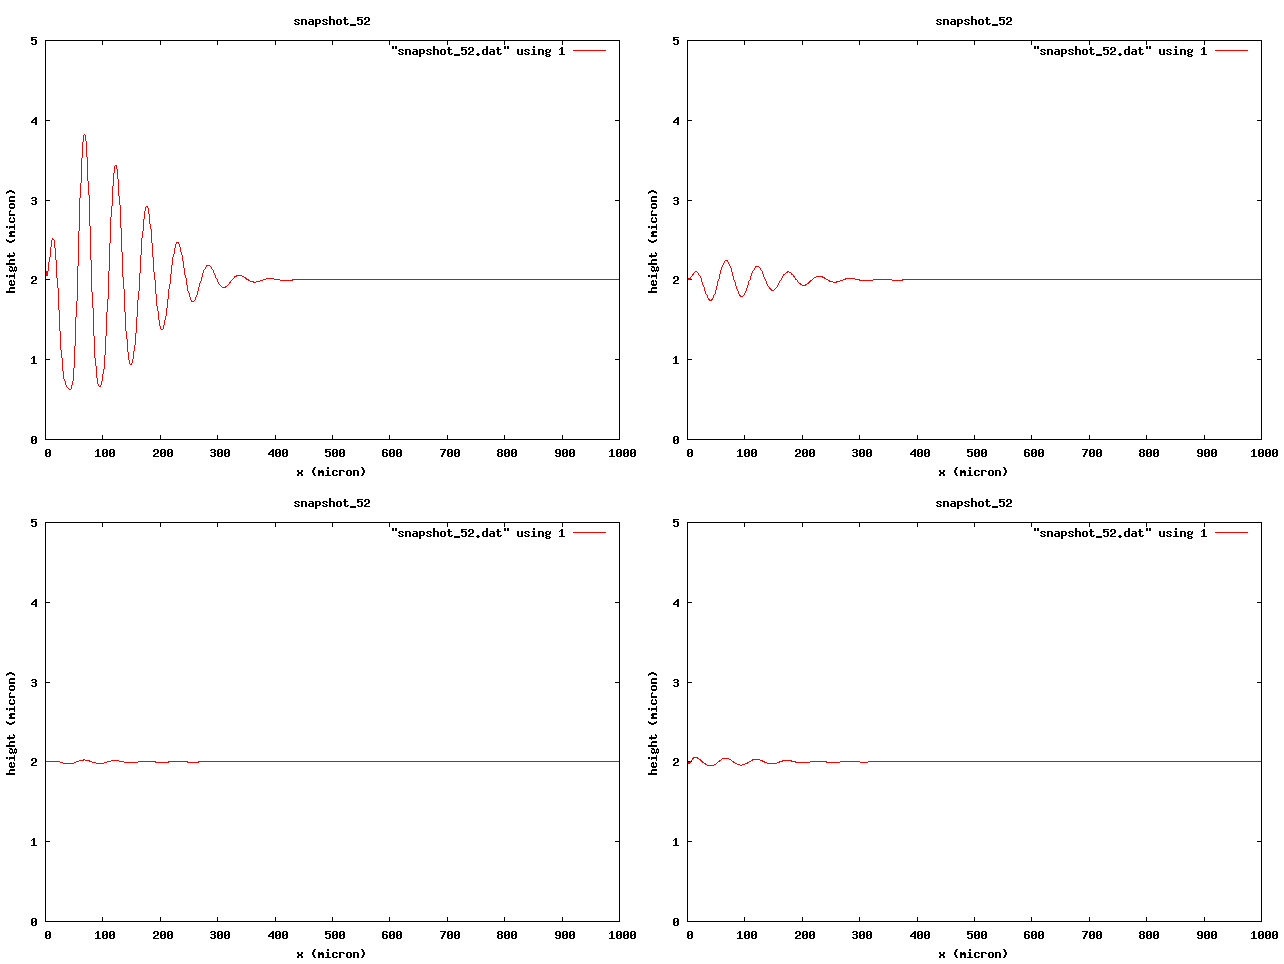
\includegraphics[width=2.45in]{figure/var_para.png}
%   \caption{Schematic diagram of surface height evolution as a function
%   of time.}
%   \label{fig:varPara}
% \end{figure}

\section{Results}
In order to test our model against a real system, we compare it to an
experiemental result on As$_2$S$_3$\cite{saliminia}. Setting $c_2 =
3c_1$ and $c_3 = 2c_1$ begins to approximate Saliminia's qualitative
description of the observed size ordering. This not only implies the
well-known anisotropy response of As$_2$S$_3$, when exposed to
extennal optical field, but also reveals the quantitative
relationship: $\epsilon_{yy} = 4\epsilon_{xx}$, $\epsilon_{xy} =
\epsilon_{xx}$.
% \footnote[1]{It does not matter that
% this scheme makes $P(x)$ negative for s-s interference since this
% serves only to change the phase of the spatial oscillations in the
% magnitude of of $\partial P(x)/ \partial x$}

\begin{table}
  \begin{ruledtabular}
                                                                                                                                                                                                                                                                                                                                                                                                                                                                                                                                \begin{tabular}{l c r}
                                                                                                                                                                                                                                                                                                                                                                                                                                                                                                                                  \textbf{Parameter}&\textbf{Meaning}&\textbf{Value}\\
                                                                                                                                                                                                                                                                                                                                                                                                                                                                                                                                  \hline
                                                                                                                                                                                                                                                                                                                                                                                                                                                                                                                                  \multicolumn{3}{c}{\textbf{Fixed Parameters}}\\
                                                                                                                                                                                                                                                                                                                                                                                                                                                                                                                                  $h_0$& Initial Thickness&2 $\mu$m\\
                                                                                                                                                                                                                                                                                                                                                                                                                                                                                                                                  $T$& Total Illumination Time&381 s\\
                                                                                                                                                                                                                                                                                                                                                                                                                                                                                                                                  $p_2$&Illumination Radius&57 $\mu$m\\
                                                                                                                                                                                                                                                                                                                                                                                                                                                                                                                                  $p_3$&Non-Oscillatory Pressure&1\\
                                                                                                                                                                                                                                                                                                                                                                                                                                                                                                                                  $p_4$&Modulation Frequency&$2\pi/13$ $\mu$m$^{-1}$\\
                                                                                                                                                                                                                                                                                                                                                                                                                                                                                                                                  $p_5$&Modulation Phase&$\pi/2$\\
                                                                                                                                                                                                                                                                                                                                                                                                                                                                                                                                  \\
                                                                                                                                                                                                                                                                                                                                                                                                                                                                                                                                  \multicolumn{3}{c}{\textbf{Free Parameters}}\\
                                                                                                                                                                                                                                                                                                                                                                                                                                                                                                                                  $p_1/\sigma$&Relative Pressure Strength&0.88 $\mu$m$^{-1}$\\
                                                                                                                                                                                                                                                                                                                                                                                                                                                                                                                                  $\sigma/\eta$&Characteristic Growth Rate&1.9$\times 10^{-3}$ $\mu$m/s\\
                                                                                                                                                                                                                                                                                                                                                                                                                                                                                                                                \end{tabular}
  \end{ruledtabular}
  \caption{Summary of the parameters used in constructing the fit depicted in figure
                                                                                                                                                                                                                                                                                                                                                                                                                                                                                                                                \ref{fig:sinemodzoom}.} \label{tab:sinemod}
\end{table}

\begin{figure}[!htbp]
  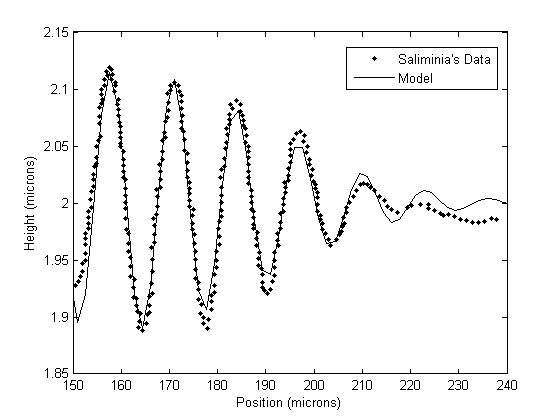
\includegraphics[width=2in]{figure/sinefigurezoom.png}
  \caption{The model's fit to a section of a surface relief profile from Saliminia's paper.}
  \label{fig:sinemodzoom}
\end{figure}

\begin{figure}[!htbp]
  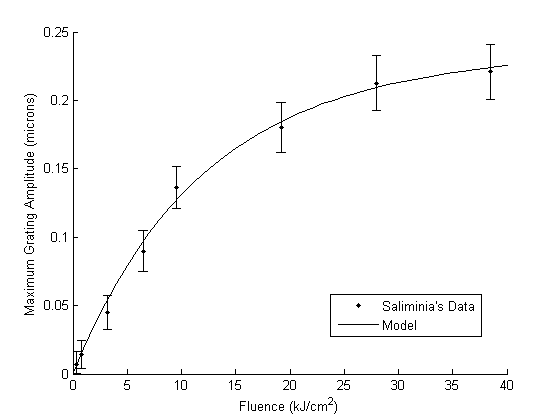
\includegraphics[width=2in]{figure/saliminiagrowth.png}
  \caption{Fluence (time) dependence of maximum surface relief amplitude for the fit in figure \ref{fig:sinemodzoom}. The $x$ axis corrects an apparent typographical error in Saliminia's original paper.}
  \label{fig:salgrowth}
\end{figure}

% \begin{figure}[!htbp]
%   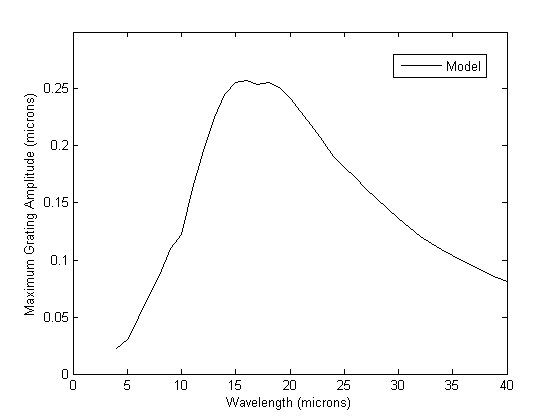
\includegraphics[width=2in]{saliminiadisp.png}
%   \caption{Dependence of the predicted maximum surface relief amplitude on spatial modulation frequency with all other parameters as in table \ref{tab:sinemod}. Although inconsistencies in Saliminia's reporting prevent a fit, the curve presented matches all the major qualitative features of Saliminia's graph.}
%   \label{fig:saldisp}
% \end{figure}

% \begin{figure}[!htbp]
%   \includegraphics[width=3in]{varPara.png}
%   \caption{Dependence of various parameters}
%   \label{fig:varPara}
% \end{figure}
% While equations \ref{eq:last} and \ref{eq:presmod} and the requirements of the numerical
% methods used specify nine constants of interest, most are set by the experimental
% procedure or the equations in table \ref{tab:theory}.
%  Of particular note are $p_1$,
% $\eta$, and $\sigma$. Rewriting the pressure as $p_1 \hat{P}(x)$ allows for the recasting
% of equation \ref{eq:last} as
% \begin{equation}
% \frac{\partial h}{\partial t} \approx \frac{\partial}{\partial x}\left(\frac{\sigma
% h^3}{3\eta}\left[\frac{p_1}{\sigma}\frac{\partial \hat{P}(x)}{\partial
% x}-\frac{\partial^3 h}{\partial x^3}\right]\right) \label{eq:fitmodel}
% \end{equation}
% which reduces the number of constants to eight and the number of fitting parameters to
% two, $\sigma/\eta$ (a material property) and $p_1/\sigma$ (the relative pressure
% strength).
The model parameters are summarized in table
\ref{tab:sinemod}. Simulation results demonstrate the consistancy
between the model and experiments. Figure \ref{fig:sinemodzoom} shows
the model's fit to a section of a surface relief profile from
Saliminia's paper. As we can see, this fit matches both the frequency
and amplitude over large space given by realistic experimental
parameters. In order to further verify the quality of
this model, we compare the time dependence as shown in figure
\ref{fig:salgrowth}. Here once again we see that with experimental
uncertainty we have a good fit to the data.
%  As can be seen from figure \ref{fig:salgrowth}, the
% fit thus produced also displays the correct time dependence. Finally,
% figure \ref{fig:saldisp} reveals that the model can account for the
% observed dependence of grating amplitude on modulation period.

% %\begin{table}\begin{center} %\begin{tabular}{|c|c|c|c|}
%\multicolumn{4}{c}{\textbf{\Large Model Parameters for the Fit in figure \ref{fig:sinemod}}}\\
%\hline
%\textbf{Parameter}&\textbf{Meaning}&\textbf{Fixed/Free} &\textbf{Value}\\
%\hline \hline
%$h_0$& Initial Thickness&Fixed&2 $\mu$m\\
%\hline
%$T$& Total Illumination Time&Fixed&381 s\\
%\hline
%$p_2$&Illumination Radius&Constrained&57 $\mu$m\\
%\hline
%$p_3$&Non-Oscillatory Pressure&Fixed&1\\
%\hline
%$p_4$&Frequency of Modulation&Fixed&$2\pi/13$ $\mu$m$^{-1}$\\
%\hline
%$p_5$&Modulation Phase&Fixed&$\pi/2$\\
%\hline
%$p_1/\sigma$&Relative Pressure Strength&Free&0.88 $\mu$m$^{-1}$\\
%\hline
%$\sigma/\eta$&Characteristic Growth Rate&Free&1.9$\times 10^{-3}$ $\mu$m/s\\
%\hline %\end{tabular} %\end{center} %\caption{Summary of the parameters used in
%constructing the fit depicted in figure \ref{fig:sinemod}.} %\label{tab:sinemod}
%\end{table}

In summary, the goal of this work was to study the mechanism of mass transport,
which results in surface morphology changes, when external stimuli are
applied to chalcogenide materials, especially As$_2$S$_3$. We applied
the Navier-Stokes equation to describe the dynamics of surface
structure change, together with a dipole interaction model to
calculate the driving force -- the optical-induced pressure. With the
derived equation of motion, simulation results are obtained, which agree
with the experiment data well and proved the validity of the model,
when it is applied chalcogenide material.

We thank XXX for assistance in preparation of the experiment, and XXX
for helpful discussions. We gratefully acknowledge support by XXX.
\bibliography{references}

\end{document}
